\documentclass[12pt,a4paper]{article}

\usepackage{style2017}
\newcounter{numexo}
\setcellgapes{1pt}
\renewcommand{\arraystretch}{1.2}
\setlength{\parskip}{0.25cm}

\begin{document}


\begin{NSI}
{Activité}{Les événements en JAVASCRIPT}
\end{NSI}

Une page WEB s'affiche sur le navigateur d'une machine cliente. On rappelle que l'affichage de cette page WEB fait suite à une requêtre HTTP de la machine cliente vers le serveur qui dispose de la page WEB.

Le serveur répond à la requête HTTP en renvoyant la page WEB demandée au format HTML et avec un code d'état égal à 200 et un statut \textsf{OK}.

La page WEB au format HTML contient des propriétés CSS pour l'affichage et aussi (éventuellement) des scripts en langage JAVASCRIPT.

\begin{center}
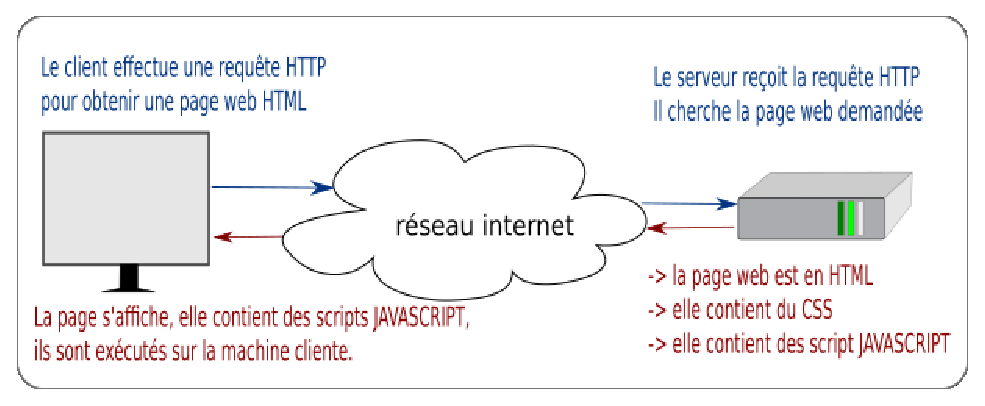
\includegraphics[scale=0.8]{img/requete_http.eps}
\end{center}

Un script JAVASCRIPT chargé avec la page web est un programme exécuté par le navigateur qui permet d'agir sur la page WEB affichée.

Un script JAVASCRIPT peut:
\begin{itemize}[label=\textbullet]
\item modifier le contenu de la page et les balises HTML.
\item modifier l'affichage en ajoutant ou modifiant les propriétés CSS,
\item interagir avec l'utilisateur avec les événements JAVASCRIPT.
\end{itemize}

Lorsqu'un script est chargé dans une fenêtre ou un onglet du navigateur, celui-ci s'exécute dans la fenêtre ou l'onglet qui l'a chargé.


Nous allons à travers quelques exemples voir et appliquer quelques scripts sur une page web. On reprendra la page WEB créée après les 2 activités précédentes.


\newpage
\section*{Introduction au JAVASCRIPT}

Un script JAVASCRIPT peut être chargé n'importe où dans la page HTML. Néanmoins, il est préférable de l'ajouter soit entre les balises \textsf{<head>} et \textsf{</head>} soit en fin de document juste avant la balise \textsf{</html>} ou la balise \textsf{</body>}.

\begin{enumerate}
\item Un script JAVASCRIPT est toujours placé entre les balises \textsf{<script text='text/javascript'>} et \textsf{</script>}.

Ajouter ces deux balises dans le head de votre document HTML.

\item On donne un premier script JAVASCRIPT à recopier.

\begin{lstlisting}
alert('un premier script');
\end{lstlisting}

\begin{enumerate}
\item Placer ce script entre les balises \textsf{<head>} et \textsf{</head>} puis actualiser la page web.
\item Déplacer ce script juste avant la balise \textsf{</body>} puis actualiser la page web.
\item Que fait ce script et quelle différence y a t-il entre les 2 positionnements ?
\end{enumerate}

\item On propose de remplacer le script précédent par celui-ci:
\begin{lstlisting}
console.log('un premier script');
\end{lstlisting}

\begin{enumerate}
\item Que se passe-t-il en actualisant la page ?
\item Ouvrir les outils de développement (F12 ou CTRL MAJ I) puis sélectionner l'onglet \textsf{Console} et afficher les journaux. Actualiser la page.
\item Modifier le texte dans le script et actualiser la page web.

\textbf{Remarque:} cette astuce est très utile pour debugger les programmes !
\end{enumerate}

\item On s'intéresse au script suivant:

\begin{lstlisting}
prompt('Quel est ton nom ?');
\end{lstlisting}

\begin{enumerate}
\item Modifier votre document HTML avec ce nouveau script puis actualiser votre page dans le navigateur.

\item Le nom saisi n'apparaît pas ! En vous aidant de la première question, ajouter une ligne de code pour afficher dans une fenêtre d'alerte le prénom saisi. Attention, il faut utiliser une variable pour mémoriser la saisie du prénom!

\item Compléter le script avec une troisième ligne pour afficher le nom en console.

\item On peut ajouter du texte avec le nom en l'insérant entre quote et concaténé avec la variable grâce au signe d'addition.

Ajouter le texte \textsf{"Votre prénom est "} pour obtenir l'affichage d'alert ci-dessous.

\begin{center}
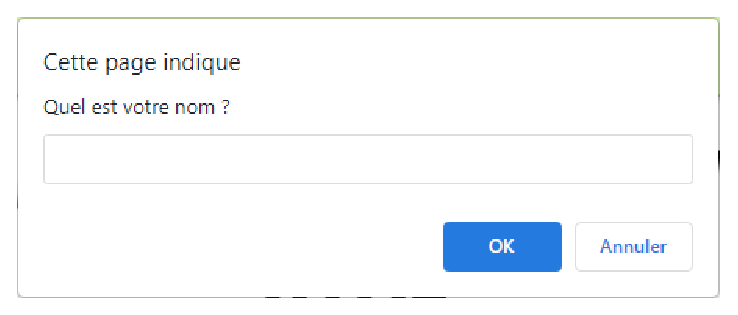
\includegraphics[scale=0.8]{img/alert_nom.eps}
\end{center}
\end{enumerate}

\end{enumerate}

\newpage

\section*{Gestion des événements en JAVASCRIPT}

Le langage JAVASCRIPT permet la gestion des événements. Il est à l'écoute des interactions de la personne avec la page WEB.

Les événements les plus courants sont:
\begin{itemize}
\item Le clic de la souris,
\item le double-clic de la souris,
\item le survol par la souris d'une partie de l'écran, d'un mot, d'une image, etc
\item le focus ou la perte de focus d'un élément de la page,
\item le chargement complet de la page,
\item la fermeture de la fenêtre.
\end{itemize}

\begin{enumerate}
\item Remplacer la balise \textsf{<script type="text/javascript">...</script>} par la balise suivante puis télécharger le fichier \textsf{script.js} disponible sur l'ENT. Ce fichier contient de petites fonctions pour agir sur le document HTML.

\begin{lstlisting}
<script type="text/javascript" src="script.js"></script>
\end{lstlisting}


\item L'événement \textsf{onclick} écoute le clic de souris dans le document WEB. Celui-ci est réservé à une zone du document.

\begin{enumerate}
\item Ajouter dans la balise \textsf{body} l'instruction suivante: \textsf{onclick="colorer()"}.

\item Recharger la page puis tester votre événement en cliquant dans le corps de la page WEB. Vous pouvez supprimer cet événement après les test.
\end{enumerate}

\item Il n'y a qu'une seule balise body ! Certaines balises sont multiples comme les titres ou les images. On peut identifier les balises par un identifiant. Un identifiant est un mot unique du document HTML qui se note dans la balise par \textsf{id="identifiant"}.

\begin{enumerate}
\item Ajouter l'identifiant \textsf{logo} dans la balise contenant le logo HTML de votre document.
\item L'événement \textsf{onmouseover} écoute le survol d'un élément HTML du document pour exécuter la fonction associée. 

Ajouter dans la balise de l'image qui a l'identifiant \textsf{logo} l'instruction \textsf{onmouseover="encadrer()"}.
\end{enumerate}

\item En HTML, on peut ajouter des boutons qui permettent de créer de l'interactivité. Pour ajouter un bouton, il faut appliquer la syntaxe suivante:

\begin{lstlisting}
<button>Texte sur le bouton</button>
\end{lstlisting}

\begin{enumerate}
\item Ajouter dans votre document HTML deux boutons. Le premier a pour texte \textsf{Alerter} et pour identifiant \textsf{btn\_1} et le second a pour texte \textsf{Saisir un nom} et pour identifiant \textsf{btn\_2}.

\item Ajouter l'événement \textsf{onclick} sur le bouton \textsf{Alerter} en associant une instruction d'alerte contenant le message "Vous êtes un lanceur d'alerte!".

\item Ajouter l'événement \textsf{onclick} sur le bouton \textsf{Saisir un nom} en associant une instruction de saisie de nom.

\end{enumerate}

\item Ouvrir avec l'éditeur \textsf{notepad++} le fichier \textsf{script.js}. Ce fichier contient des fonctions écrites en javascript qui vont nous servir de modèle.

\begin{enumerate}
\item Compléter la fonction \textsf{alerter} pour afficher le message "Vous êtes un lanceur d'alerte!" puis associer cette fonction au bouton \textsf{btn\_1}.

\item Compléter la fonction \textsf{saisir\_nom} pour provoquer la saisie du nom puis associer cette fonction au bouton \textsf{btn\_2}.

\item Modifier les deux fonctions précédentes pour afficher le message et le nom saisi en console.
\end{enumerate}

\end{enumerate}

\end{document}

